\documentclass[a4paper]{exercisesheet}

%\usepackage{mathpazo}
%\usepackage{mathptmx}
%\usepackage{newtxmath}
\usepackage[T1]{fontenc}
\usepackage[utf8]{luainputenc}
\usepackage[charter]{mathdesign}
\let\sfdefault=\rmdefault
\def\ttdefault{txtt}

\usepackage{graphicx}

\usepackage[dvipsnames]{xcolor}
%\colorlet{maincolor}{blue!50!black}
\colorlet{maincolor}{black}

\usepackage{listings}
\usepackage{amsmath}
%\lstset{
%  frame=lines,
%  backgroundcolor=\color{maincolor!15},
%  rulecolor=\color{maincolor},
%  language=Python
%  keywordstyle=\bfseries\color{maincolor},
%  numbers=left,
%  numberstyle=\scriptsize\color{maincolor!70},
%}

\linespread{1.04}

\usepackage[english]{babel}

\usepackage{blindtext}

\sheetconf{
    lecture   = {Networks and Complex Systems},
  lecturer  = {F.~Klimm~und~B.F.~Maier},
  semester  = {Sch\"ulerakademie 5.2 (Ro\ss leben 2016)},
  author    = {},
  % teacher,
  solutions=false,
}

\setsheetfont{lecture on titlepage}{\sffamily\Huge}
\setsheetfont{sheet title}{\sffamily\Large}
\setsheetfont{type on titlepage}{\sffamily\scriptsize\color{maincolor}}
\setsheetfont{sheet topic}{\sffamily\Huge\color{maincolor}}
\setsheetfont{sheet lecture}{\it\sffamily\Large\color{maincolor}}
\setsheetfont{exercise topic}{\sffamily\Large\color{maincolor}}
\setsheetfont{exercise label}{\sffamily\Large\color{maincolor}}
\setsheetfont{subexercise topic}{\sffamily\large\color{maincolor}}
\setsheetfont{subexercise label}{\sffamily\large\color{maincolor}}

\setsheettemplate{sheet title (student)}{Worksheet~\thesheet}
\setsheettemplate{exercise name}{Exercise}
\setsheettemplate{subexercise name}{Subexercise}

\lstset{%
  %linewidth=\textwidth,
  %linewidth=16cm,
  language=Python,                  % the language of the code
  basicstyle=\ttfamily\small,
  backgroundcolor=\color{maincolor!5},
  %basicstyle=\footnotesize,      % the size of the fonts that are used for the code
  numbers=left,                   % where to put the line-numbers
  stepnumber=1,                   % the step between two line-numbers. If it's 1, each line 
                                  % will be numbered
  numberstyle=\scriptsize\color{maincolor!70},
  numbersep=5pt,                  % how far the line-numbers are from the code
  frame=single,                   % adds a frame around the code
  rulecolor=\color{black},        % if not set, the frame-color may be changed on line-breaks
  tabsize=4,                      % sets default tabsize to 2 spaces
  captionpos=b,                   % sets the caption-position to bottom
  breaklines=true,                % sets automatic line breaking
  breakatwhitespace=false,        % sets if automatic breaks should only happen at whitespace
  %keywordstyle=\color{blue},      % keyword style
  %commentstyle=\color{dkgreen},   % comment style
  %stringstyle=\color{colorNavy},  % string literal style
  morekeywords={*,with, where, from, union, all, as},
  extendedchars=true,
  literate={ä}{{\"{a}}}1 {ö}{{\"o}}1 {ü}{{\"u}}1,
}


\begin{document}

  \sheet[%
  number=3,
  topic={Matrix Calculations and Effective Resistance},
      %deadline=Deadline: \today,
    ]


\vspace{-1cm}
\noindent\rule{12cm}{0.4pt}

  \exercise[%
  topic = Matrix multiplication
  ]
  Let $\hat P$ denote the reproduction matrix of a system of linearly
  interacting sheep, wolves and units of pasture with
  \begin{equation}
      \hat P = 
      \left(
      \begin{matrix}
          1    & -0.1   & 0.1 \\
          0.1  & 0.9 & 0 \\
          -0.1 & 0   & 1.1 
      \end{matrix}
  \right).
   \end{equation}
   This matrix encodes how the abundances of the species develop in one month.
   
 \subexercise[%
  topic={Population growth},
    ]

   The current abundance of species is given by the population vector
   \begin{equation}
       \label{eq:equalpop}
       \vec x_0 = \left(\begin{matrix}
               10\\
               10\\
               10
           \end{matrix}\right).
   \end{equation}
   Calculate the population vector in one month.

 \subexercise[%
  topic={Matrix inversion},
    ]
    \emph{Introduction)}
    Some squared matrices $\hat A$ possess a so-called \textit{inverse}
    $\hat A^{-1}$ which fulfills
    \begin{equation}
        \hat A \cdot \hat A^{-1} = \hat A^{-1}\cdot \hat A = 1\!\!\!1,
    \end{equation}
    with the identity matrix
    \begin{equation}
        1\!\!\!1 = \left(\begin{matrix}
                1 & 0 & 0& \ & 0\\
                0 & 1 & 0&\dots & 0\\
                0 & 0 & 1 &\ & 0\\
                \vdots & \ & \ & \ddots & 0\\
                0 & 0 & 0 & 0 & 1 
            \end{matrix}\right).
    \end{equation}
    Show that two-dimensional matrizen
    \begin{equation}
        \hat A = \left(\begin{matrix} a & b \\ c & d
            \end{matrix}\right)
    \end{equation}
    posses the inverse
    \begin{equation}
        \hat A = \frac{1}{ad-bc}\left(\begin{matrix} d & -b \\ -c & a
            \end{matrix}\right).
    \end{equation}
    Let
    \begin{equation}
        \hat R = \left(\begin{matrix} 1 & 1 \\ -1 & 1
            \end{matrix}\right)
    \end{equation}
    denote the reproduction matrix of a sheep-wolf-system.
    The current population vector is
   \begin{equation}
       \vec x_1 = \left(\begin{matrix}
               97\\
               37
           \end{matrix}\right).
   \end{equation}
   What was the population vector one month ago?
 
   \emph{Exercise)}\ Given the reproduction matrix $\hat P$ and the
   current population vector
   \begin{equation}
       \vec x_1 = \left(\begin{matrix}
               37\\
               49\\
               18
           \end{matrix}\right).
   \end{equation}
   What was the population vector one month ago?

 \subexercise[%
     topic={Eigenpopulations},
    ]

    Let the reproduction matrix be

  \begin{equation}
      \hat Q = 
      \left(
      \begin{matrix}
          1    & -0.5   & -0.5 \\
          -1  & 1 & 0 \\
          -1  & 0   & 1 
      \end{matrix}
  \right).
   \end{equation}
   Given the population from equation \ref{eq:equalpop}, calculate the
   population vector in one month. Is $\vec x_0$ an eigenvector of $\hat
   Q$? If this is the case, which is  eigenvalue corresponding to this
   eigenvector of $\hat Q$?

   Given the two-dimensional reproduction matrix
  \begin{equation}
      \hat Q_2 = 
      \left(
      \begin{matrix}
          1    & -1 \\
          -1  & 1
      \end{matrix}
  \right)
   \end{equation}
   and an initial population of 10 sheep and 10 wolves, calculate the
   population after a month. What is the corresponding eigenvalue of
   this population? What does that mean for the inverse matrix
   $\hat Q_2^{-1}$?
   
    \subexercise[%
     topic={Inverse of a Singular Matrix},
    ]
    Prove the following theorem.\ \\

    L $\hat A$ be a square matrix with eigenvalue where none of the
    corresponding eigenvectors are the null vector. Then, $\hat A$ is
    not invertible.

    Such a matrix is called ``singular''.


  \exercise[%
  topic = {Effective Resistance}
  ]

 \subexercise[%
  topic={Calculate},
    ]

  Take a look at figure \ref{resistors}. What is the effective
  resistance of the network between nodes $s$ and $t$?

\begin{figure}[h]
\centering{
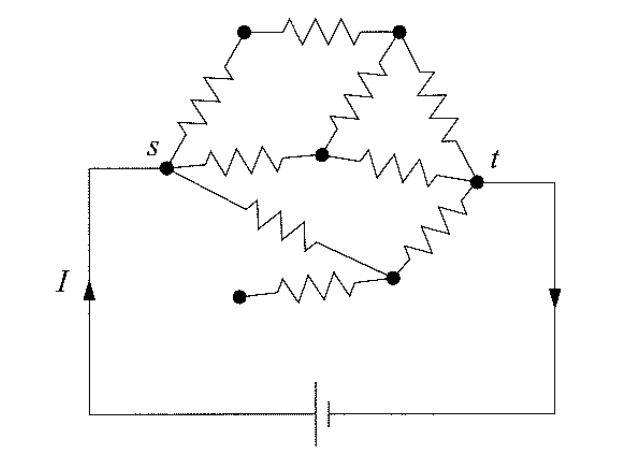
\includegraphics[width=0.5\textwidth]{resistornetwork.png}
   \caption{\label{resistors} A resistor network. In this 
       circuit we have the electric current $I$ and all resistors 
       carry resistance
        $R_0$. Figure taken from ``Networks -- An Introdution'', M. Newman,
    Oxford University Press, 2010, p. 162. 
        }
    }
\end{figure}


 \subexercise[%
  topic={General Networks of Resistors $R_0$}
    ]

    Write a Python function which takes the adjacency matrix $\hat A$,
    the input node $s$ and the output node $t$ as input and calculates
    and returns the effective resistance of the network.
    berechnet.

    Investigate the relationship between the effective resistance between any
    two nodes of a random graph and the number of nodes $n$ as well as
    the connection probability $p$.



 \exercise[%
     topic={Extra) Percolation of Random Graphs},
    ]
     Find out how to find the components of a network.

     Write a Python function doing exactly that for arbitrary networks.

     Generate random graphs for varying node numbers $n$ and connection
     probabilities $p$ and find the normed ratio $S$ of the largest
     component, where $S=|V_g|/n$ with the number of nodes $|V_g|$ in
     the largest component (component with node and edge sets
     $(V_g,E_g)$).

     Investigate, how $S$ is influenced by increasing $p$ for constant
     $n$. What is the critical probability $p_c$ for the existence of a
     giant component? What is the mean degree?

    
     Increase $n$. How does $p_c$ change? Can you find a formula for
     $p_c$ for arbitrary $n$ and $p$?

     How do you interpret this formula?
	
\end{document}
